\begin{figure*}[!h]
\begin{subfigure}{0.23\linewidth}
\centering
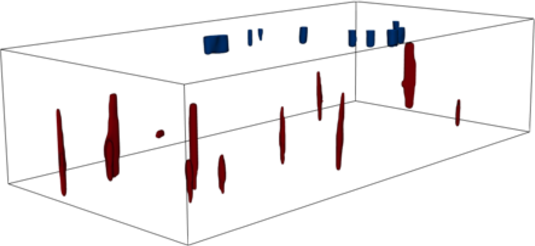
\includegraphics[width=\linewidth]{Images/Mantel/zls.pdf}
\vspace{-5mm}
\caption{$ZLS_{T}$}
\label{fig:mantel_zls}
\end{subfigure}
\begin{subfigure}{0.23\linewidth}
\centering
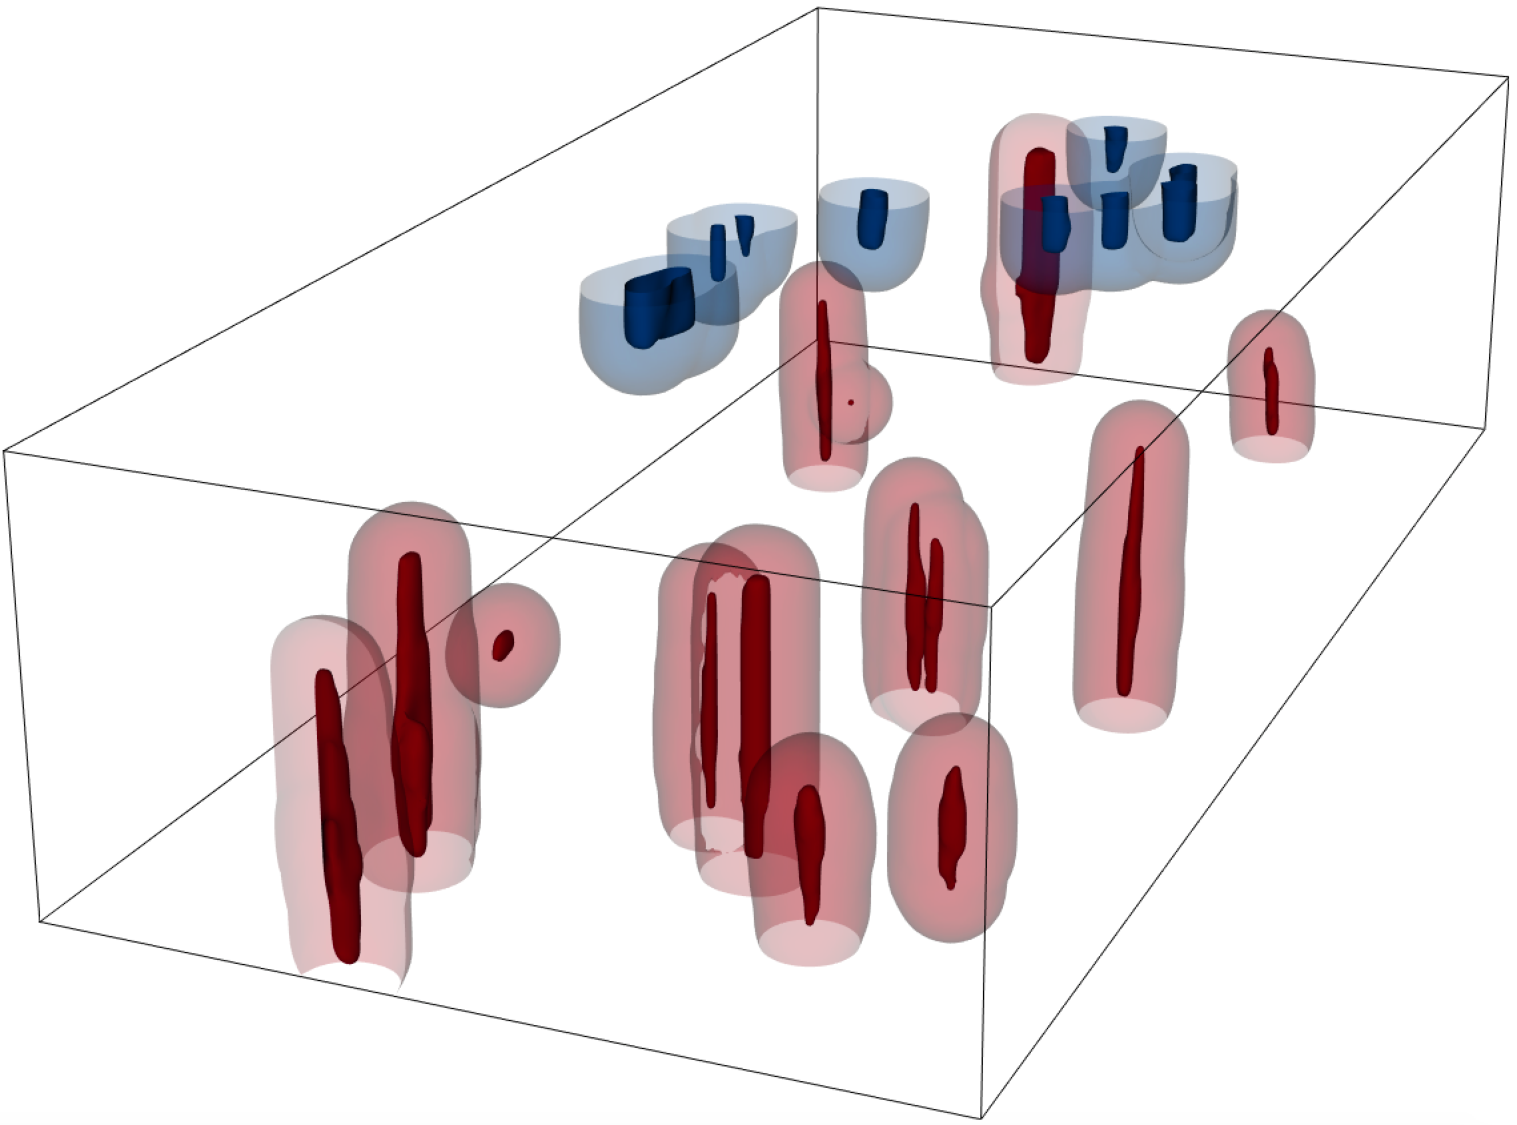
\includegraphics[width=\linewidth]{Images/Mantel/fls_10.pdf}
\vspace{-5mm}
\caption{$ZLS_{T}$ + $FLS_{T,10}$}
\label{fig:mantel_fls}
\end{subfigure}
\begin{subfigure}{0.23\linewidth}
\centering
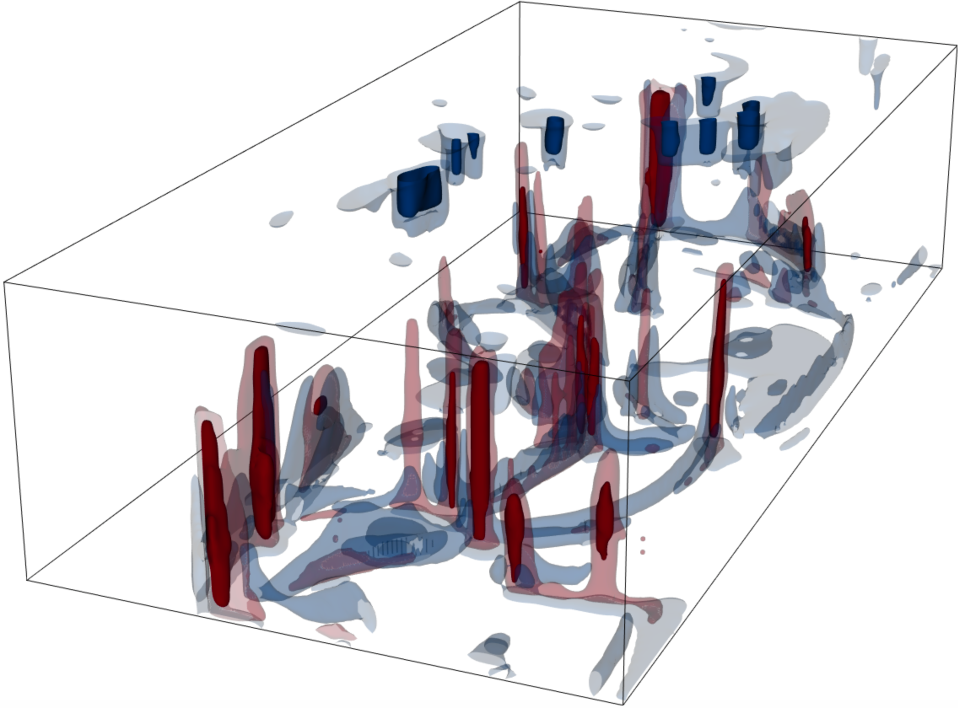
\includegraphics[width=\linewidth]{Images/Mantel/fcls_68.pdf}
\vspace{-5mm}
\caption{$ZLS_{T}$ + $FCLS_{T,68\%}$}
\label{fig:mantel_fcls}
\end{subfigure}
\hfill
\begin{subfigure}{0.28\linewidth}
\centering
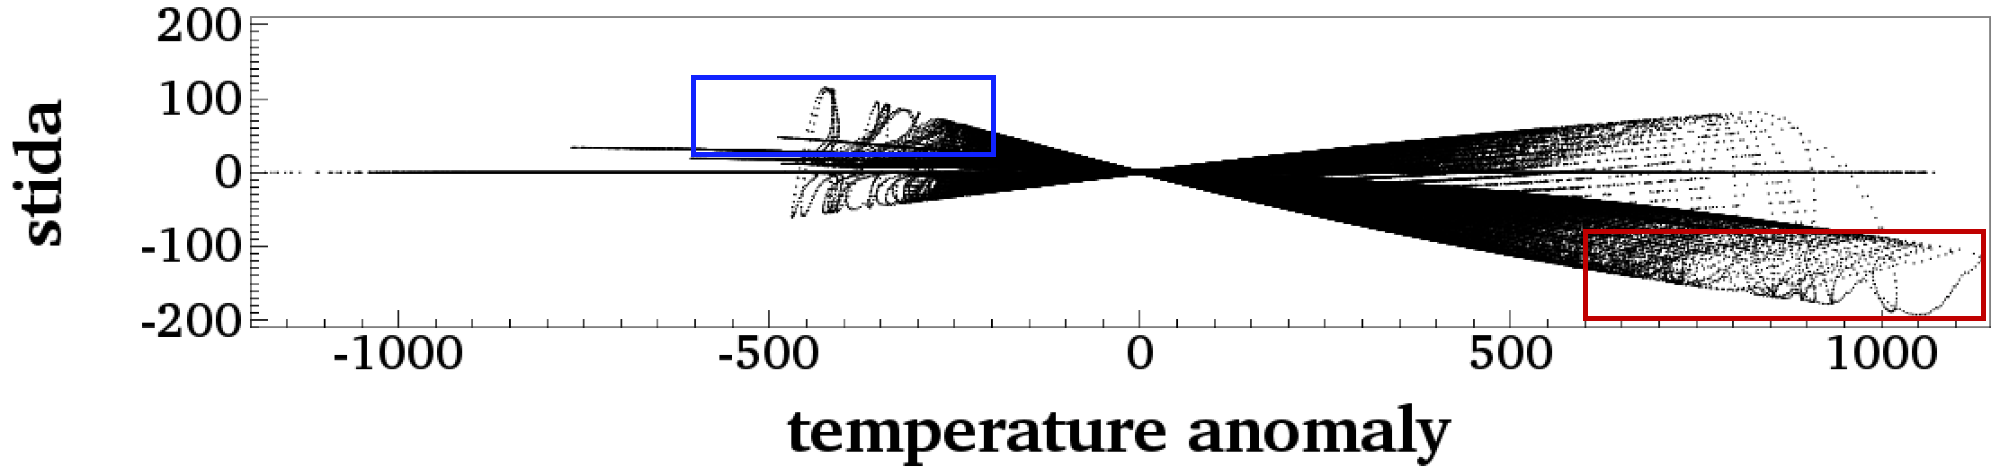
\includegraphics[width=\linewidth]{Images/Mantel/scatterplot.pdf}
%\vspace{-2mm}
\caption{Attribute space 2D scatterplot and, traits (labeled rectangular selections). We use $T = \left\{T_{A}, T_{B}\right\}$.} 
\label{fig:mantel_scatterplot}
\end{subfigure}
\vspace{-3mm}
\caption{Visualization of rising hot plumes~($T_{A}$, red) and sinking material~($T_{B}$, blue) flow patterns in a subset of the spatial domain for the mantel data using the temperature anomaly and spin transition induced density anomaly~(stida) attributes.}
\label{fig:mantel}
\end{figure*}
